\section{Spannungsregler/Stromversorgung\hartl{280}} 
\subsection{Lineare Spannungsregler\hartl{280}} 
Für alle linearen Spannungsregler gilt: \begin{equation*}
P_{V}=(V_{E}-V_{a})*I_{a}
\end{equation*}\\
Einsatz für geringer Spannungsunterschied zwischen eingangsspannung und der
geregelten Ausgangsspannung

\begin{longtable}{|l|l|l|}
\hline
\begin{minipage}{4cm}
\textbf{Spannungs-stabilisierung mit Transistor} \hartl{280}
\end{minipage}
&
\begin{minipage}{6cm}
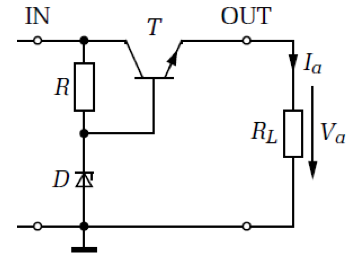
\includegraphics[width=6cm, height =
4cm]{pictures/transistorStabilisierung}
\end{minipage}
&
\begin{minipage}{8cm}
\begin{gather*}
I_{E}=I_{L}\approx I_{C}\\
U_{E}=U_{A}+U_{CE}\\
U_{A}=U{Z}-U_{BE}\\
R_{V}=\frac{U_{E}-U_{Z}}{I_{Z}+I_{B}}\\
I_{B}=\frac{I_{C}}{B}\\
R_{i}\approx\frac{r_{Z}}{\beta} 
\end{gather*}
\begin{tabular}{ll}
$U_{E}$:&unstab. Eingangsspannung\\
$U_{A}$:&stab. Ausgangsspannung\\
$U_{Z}$:&ZDioden-Spannung\\
$U_{CE}$:&Kollektor-Emitterspannung\\
$U_{BE}$:&Basis-Emitterspannung\\
$I_{Z}$:&Strom durch die Z-Diode\\
$I_{C}$:&Kollektorstrom\\
$I_{B}$:&Basisstrom\\
$B$:&Gleichstromverstärkung\\
$R_{i}$:&Innenwiderstand der Schaltung\\
$r_{Z}$:&dyn. Innenwiderstand der Z-Diode\\
$\beta$:&Stromverstärkungsfaktor des \\&Transistors
\end{tabular}
\end{minipage}
\\
\hline
\begin{minipage}{4cm}
\textbf{Festspannungsregler} \hartl{282}
\end{minipage}
&
\begin{minipage}{6cm}
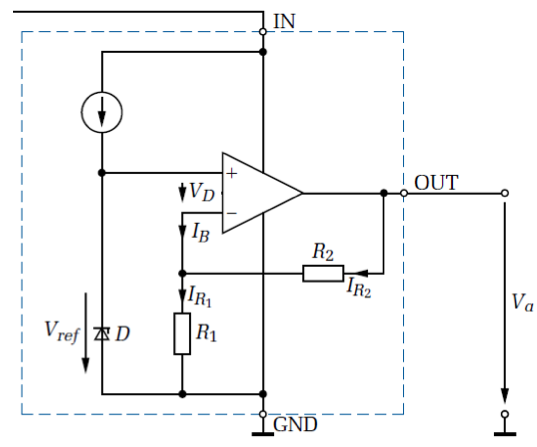
\includegraphics[width=6cm, height =
4cm]{pictures/festStabilisierung}
\end{minipage}
&
\begin{minipage}{8cm}
\begin{gather*}
V_{ref}=V_{D}+V_{R1}\\
V_{a}=I*(R_{2}+R_{1})=\frac{V_{ref}}{r}*4R=4*V_{ref}
\end{gather*}
\end{minipage}
\\
\hline
\begin{minipage}{4cm}
\textbf{Festspannungsregler mit einstellbarer Ausgangsspannung} \hartl{284}
\end{minipage}
&
\begin{minipage}{6cm}
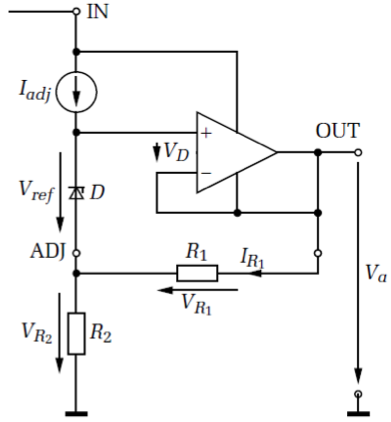
\includegraphics[width=6cm, height =
4cm]{pictures/einstellbarStabilisierung}
\end{minipage}
&
\begin{minipage}{8cm}
\begin{gather*}
V_{a}=V_{R1}+V_{R2}=V_{ref}+R_{2}*(I_{R1}+I_{adj})=\notag\\=V_{ref}+R_{2}*(\frac{V_{ref}}{R_{1}}+I_{adj})\\
\text{für }I_{adj}<< I_{R1} \to V_{a}=V_{ref}*(1+\frac{R_{2}}{R_{1}})
\end{gather*}
\end{minipage}
\\
\hline
\end{longtable}

\subsection{Schaltregler\hartl{285}} 
\begin{longtable}{|l|l|l|}
\hline
\begin{minipage}{4cm}
\textbf{Abwärtswandler (Buck Converter)} \hartl{285}
\end{minipage}
&
\begin{minipage}{6cm}
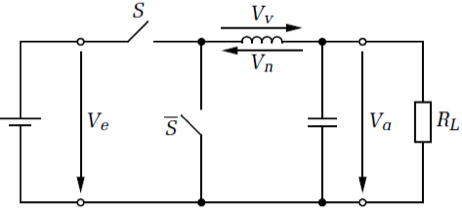
\includegraphics[width=6cm, height =4cm]{pictures/abwaertsWandler}
\end{minipage}
&
\begin{minipage}{8cm}
Es gilt: $0\leq V_{a}\leq V_{e}$\\
\begin{gather*}
S_{on}\notag\\
V_{V}=L*\frac{\Delta I_{L}}{\Delta t}\\
V_{e}=V_{V}+V_{a} \to V_{e}=L*\frac{\Delta I_{L}}{\Delta t}+V_{a}\\
S_{off}\notag\\
V_{n}=V_{a}=L*\frac{\Delta I_{L}}{\Delta t}\\
\Delta I_{L}=(V_{e}-V_{a})*\frac{1}{L}*t_{ein}\\
V_{a}=\frac{t_{ein}}{t_{aus}+t_{ein}}*V_{e}=d*V_{e}
\end{gather*}
\begin{tabular}{ll}
d:&Tastverhältnis/Duty Factor\\
\end{tabular}
\end{minipage}
\\
\hline
\begin{minipage}{4cm}
\textbf{Aufwärtswandler (Boost Converter)} \hartl{288}
\end{minipage}
&
\begin{minipage}{6cm}
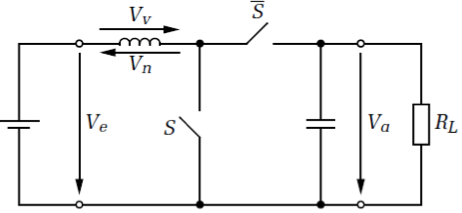
\includegraphics[width=6cm, height =4cm]{pictures/aufwaertsWandler}
\end{minipage}
&
\begin{minipage}{8cm}
Es gilt : $V_{a}\geq V_{e}$\\
\begin{gather*}
S_{on}\notag\\
V_{v}=V_{e}=L*\frac{\Delta I_{L}}{\Delta t}\\
S_{off}\notag\\
V_{a}=V_{e}+V_{n}= L*\frac{\Delta I_{L}}{\Delta t}+V_{e}\\
\Delta I=\frac{1}{L}*V_{e}*t_{ein}\\
\Delta I=\frac{1}{L}*(V_{a}-V_{e})*t_{aus}\\
V_{a}=V_{e}\frac{t_{ein}+t_{aus}}{t_{aus}}=V_{e}\frac{1}{1-d}\notag\\\text{mit
}d=\frac{t_{ein}}{t_{aus}+t_{ein}}\\
\text{Energie im Magnetfeld:}\\
E_{L}=0.5L*ipk^2
\end{gather*}
\end{minipage}
\\
\hline
\begin{minipage}{4cm}
\textbf{Invertierender Wandler (Buck Boost Converter)} \hartl{289}
\end{minipage}
&
\begin{minipage}{6cm}
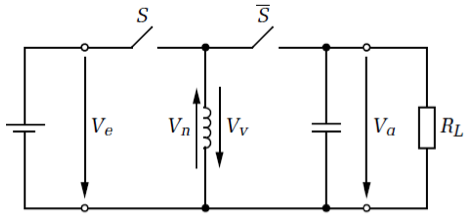
\includegraphics[width=6cm, height =4cm]{pictures/inventierenderWandler}
\end{minipage}
&
\begin{minipage}{8cm}
\begin{gather*}
S_{on}\notag\\
V_{v}=V_{e}=L*\frac{\Delta I_{L}}{\Delta t}\\
S_{off}\notag\\
V_{a}=-V_{n}=-L*\frac{\Delta I_{L}}{\Delta t}\\
V_{a}=-V_{e}*\frac{t_{ein}}{t_{aus}}=-V_{e}*\frac{d}{1-d} \notag\\\text{mit
}d=\frac{t_{ein}}{t_{aus}+t_{ein}}
\end{gather*}
\end{minipage}
\\
\hline
\end{longtable}

\subsection{Regelung der Ausgangsspannung: Voltage Mode}
\begin{itemize}
  \item Mit PWM-Signal
  \item Ist Vout zu klein, wird Ladezeit (damit Strom) erhöht $\to V_{out}$wird
  grösser
\end{itemize}
\begin{figure}[htbs]
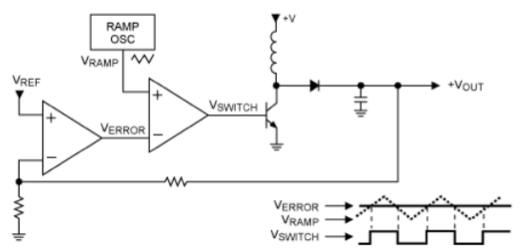
\includegraphics[scale=0.5]{pictures/ausgangsspannungsregelung}
\end{figure}

\subsection{Regelung mit Current mode}
\begin{itemize}
  \item Strom und Spannung werden gemessen
  \item Innerer Loop muss schneller sein als äusserer Loop
\end{itemize}
\begin{figure}[htbs]
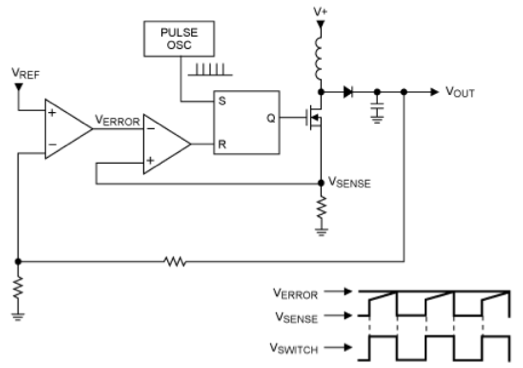
\includegraphics[scale=0.5]{pictures/currentmode}
\end{figure}

\subsection{Effizienzsteigerung}
\subsubsection{MOSFET statt Diode}
\begin{figure}[htbs]
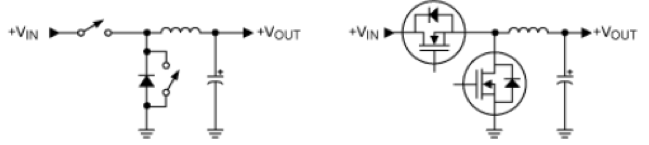
\includegraphics[scale=0.5]{pictures/effizient1}
\end{figure}
\begin{itemize}
  \item Diode hat Spannungsabfall
  \begin{itemize}
    \item Silizium-Diode: 0.7V
    \item Schottky-Diode: 0.3V
    \item MOSFET hat "`nur"' On-Widerstand $Rds_{on}$
    \end{itemize}
   \item Umschalten vom Substratpotential beim Längstransistor nötig
   \begin{itemize}
     \item Synchronous rectifier
    \end{itemize}
\end{itemize}

\subsubsection{Skip-Mode}
\begin{figure}[htbs]
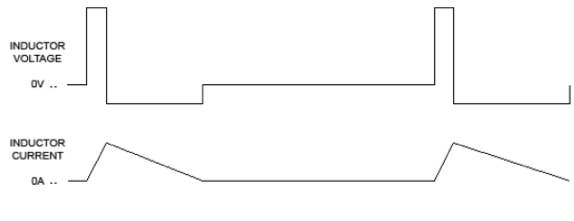
\includegraphics[scale=0.5]{pictures/effizient2}
\end{figure}
\begin{itemize}
  \item Lade- und Entladezyklen werden ausgelassen bei niedrigem Laststrom
\end{itemize}
